\documentclass[tikz, border=2pt]{standalone}
\usepackage{amsmath}

\begin{document}
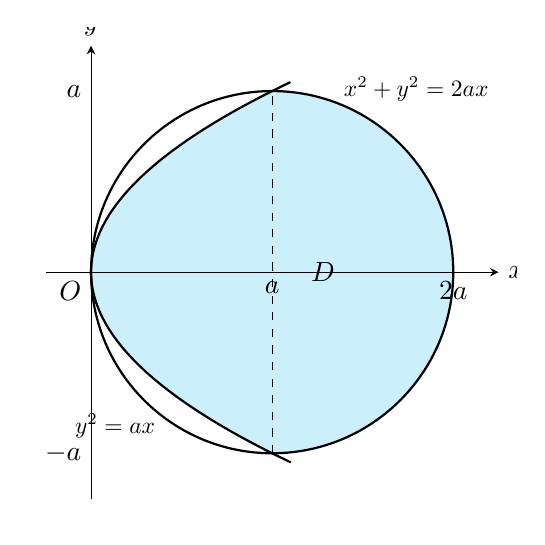
\begin{tikzpicture}[scale=2.3, >=stealth]
    % Draw with a=1: circle x^2+y^2=2x and parabola y^2=x.
    \clip (-0.35,-1.35) rectangle (2.35,1.35);
    \fill[cyan!20]
      plot[variable=\t, domain=-1:1, samples=100] ({\t*\t},{\t})
      -- plot[variable=\t, domain=1:-1, samples=120] ({1+sqrt(1-\t*\t)},{\t})
      -- cycle;

    \draw[->] (-0.25,0) -- (2.25,0) node[right] {$x$};
    \draw[->] (0,-1.25) -- (0,1.25) node[above] {$y$};

    \draw[thick] (1,0) circle (1);
    \draw[thick, variable=\t, domain=-1.05:1.05, samples=120] plot ({\t*\t},{\t});

    \draw[dashed] (1,-1) -- (1,1);
    \node[below left] at (0,0) {$O$};
    \node[below] at (1,0) {$a$};
    \node[below] at (2,0) {$2a$};
    \node[left] at (0,1) {$a$};
    \node[left] at (0,-1) {$-a$};
    \node[above right, scale=0.85] at (1.35,0.9) {$x^2+y^2=2ax$};
    \node[left, scale=0.85] at (0.4,-0.85) {$y^2=ax$};
    \node at (1.28,0) {$D$};
\end{tikzpicture}
\end{document}
